\chapter{A energia no dia a dia}\label{ch:g5:everyday-energy}

Um brinquedo de corda corre pelo chão, vai perdendo velocidade e
para --- até você dar corda de novo. Uma lanterna vai enfraquecendo
conforme as \omterm{def:g3:first-electric-circuit:battery}{pilhas} cansam. Você mesmo fica sem \omterm{def:g3:solids-liquids-gases:gas}{gás} antes do almoço.
Tudo o que se move, brilha, soa ou esquenta parece estar gastando
alguma coisa. A física tem um nome para essa coisa, e ele talvez seja
a palavra mais importante deste livro inteiro: \omterm{def:g5:everyday-energy:energy}{energia}.

\section{A coisa que faz acontecer}

\begin{definition}[Energia]\label{def:g5:everyday-energy:energy}
\emph{Energia}\index{energia} é aquilo de que se precisa para fazer
as coisas acontecerem: pôr coisas em movimento, levantá-las,
iluminá-las, aquecê-las, fazê-las soar. Nada anda, brilha ou cresce
sem que se gaste energia nisso --- e quem está gastando precisa,
antes, ter energia para gastar.
\end{definition}

\begin{definition}[Reservas de energia]\label{def:g5:everyday-energy:store}
Uma \emph{reserva de energia}\index{reserva de energia} é qualquer
coisa que guarda \omterm{def:g5:everyday-energy:energy}{energia} pronta para ser usada. As grandes reservas
do dia a dia: o \emph{alimento} (o combustível do seu corpo), os
\emph{combustíveis} como a lenha e a gasolina, as \emph{\omterm{def:g3:first-electric-circuit:battery}{pilhas}}
carregadas, uma \emph{mola} com corda, a água represada \emph{lá em
cima} atrás de uma barragem --- e o Sol quente, despejando \omterm{def:g5:everyday-energy:energy}{energia}
sobre tudo, o dia inteiro, de graça.
\end{definition}

\begin{example}[Ache a reserva]\label{ex:g5:everyday-energy:spot}
Toda coisa que anda tem uma reserva por trás dela. O brinquedo que
corre: a mola com corda. A lanterna: as \omterm{def:g3:first-electric-circuit:battery}{pilhas}. O carro: o
combustível do tanque. Você: o seu café da manhã. O veleiro: o \omterm{def:g2:air-around-us:air}{ar} em
movimento do \omterm{def:g2:air-around-us:wind}{vento}. Quando a reserva se esvazia --- mola sem corda,
\omterm{def:g3:first-electric-circuit:battery}{pilhas} descarregadas, tanque seco, hora do almoço chegando --- o
andar para.
\end{example}

\begin{remark}[Sem alimentar, sem andar]\label{rem:g5:everyday-energy:nofree}
Durante séculos, inventores caçaram máquinas que funcionassem para
sempre sem nada --- rodas que giram sozinhas, relógios que nunca
precisam de corda. Todas, sem exceção, fracassaram. Esse fracasso é
uma das lições mais profundas da física: a \omterm{def:g5:everyday-energy:energy}{energia} nunca é
conjurada do nada. Tudo o que funciona está sendo alimentado --- ache
a reserva e você entende a máquina.
\end{remark}

\section{A energia muda de forma}

\begin{example}[Formas de energia]\label{ex:g5:everyday-energy:forms}
A \omterm{def:g5:everyday-energy:energy}{energia} se mostra em formas diferentes: \omterm{def:g5:everyday-energy:energy}{energia} de
\emph{movimento} na bola que rola e no \omterm{def:g2:air-around-us:wind}{vento} que sopra; \omterm{def:g5:everyday-energy:energy}{energia} de
\emph{\omterm{def:g1:light-and-shadows:source}{luz}} jorrando da lâmpada e do Sol; \omterm{def:g5:everyday-energy:energy}{energia} de \emph{calor} em
tudo o que está quente; \omterm{def:g5:everyday-energy:energy}{energia} \emph{elétrica} viajando pelos fios;
\omterm{def:g5:everyday-energy:energy}{energia} \emph{armazenada} esperando quietinha nos alimentos, nos
combustíveis, nas molas e nas coisas levantadas. A mesma coisa,
muitas formas.
\end{example}

\begin{proposition}[A cadeia da energia]\label{prop:g5:everyday-energy:chain}
Sempre que alguma coisa acontece, a \omterm{def:g5:everyday-energy:energy}{energia} é tirada de uma reserva e
passada adiante, em geral mudando de forma no caminho. Ela nunca é
criada do nada --- e também nunca é realmente destruída: aquilo que
uma máquina ``gasta'' apenas foi passado adiante, terminando quase
sempre, mais cedo ou mais tarde, como um calorzinho espalhado pelo
ambiente.
\end{proposition}

\begin{method}[Ler uma cadeia de energia]\label{met:g5:everyday-energy:read}
Para entender qualquer aparelho, siga a cadeia dele:
\begin{enumerate}
  \item ache a \emph{reserva} de onde vem a \omterm{def:g5:everyday-energy:energy}{energia};
  \item ache o \emph{conversor} --- a parte em que a \omterm{def:g5:everyday-energy:energy}{energia} muda de
        forma;
  \item diga as formas que saem --- a útil e o calor que vaza junto.
\end{enumerate}
A lanterna, seguida assim: \omterm{def:g3:first-electric-circuit:battery}{pilha} (reserva) $\to$ lâmpada (conversor)
$\to$ \omterm{def:g1:light-and-shadows:source}{luz} (útil) $+$ um pouquinho de calor (a perda --- encoste na
lâmpada).
\end{method}

\begin{omfigure}
\begin{tikzpicture}[scale=0.85]
  \node[draw, thick, omDef, font=\small, minimum width=2.5cm,
    minimum height=0.9cm] (a) at (1.4,0) {pilha: reserva};
  \node[draw, thick, omMeth, font=\small, minimum width=2.5cm,
    minimum height=0.9cm] (b) at (5.4,0) {lâmpada: conversor};
  \node[draw, thick, omThm, font=\small, minimum width=2.2cm,
    minimum height=0.9cm] (c) at (9.4,0.7) {luz: útil};
  \node[draw, thick, omExo, font=\small, minimum width=2.2cm,
    minimum height=0.9cm] (d) at (9.4,-0.7) {calor: perda};
  \draw[-Stealth, very thick] (a) -- (b);
  \draw[-Stealth, very thick] (b) -- (c);
  \draw[-Stealth, very thick] (b) -- (d);
\end{tikzpicture}

{\small A cadeia de \omterm{def:g5:everyday-energy:energy}{energia} da lanterna: a \omterm{def:g5:everyday-energy:energy}{energia} armazenada vira
\omterm{def:g1:light-and-shadows:source}{luz} --- e um pouquinho de calor sempre escapa junto.}
\end{omfigure}

\begin{example}[Cadeias em toda parte]\label{ex:g5:everyday-energy:chains}
O seu passeio de manhã, seguido: café da manhã (reserva) $\to$ os
seus músculos (conversor) $\to$ movimento da bicicleta $+$ calor
(você sente --- você fica quente). O parque eólico: \omterm{def:g2:air-around-us:air}{ar} em movimento
$\to$ pás girando $\to$ \omterm{def:g5:everyday-energy:energy}{energia} elétrica nos fios $\to$ \omterm{def:g1:light-and-shadows:source}{luz} na sua
luminária hoje à noite. A barragem: água lá em cima $\to$ a água
caindo gira as turbinas $\to$ \omterm{def:g5:everyday-energy:energy}{energia} elétrica. As cadeias longas são
só cadeias curtas emendadas: forma depois de forma depois de forma.
\end{example}

\begin{omfigure}
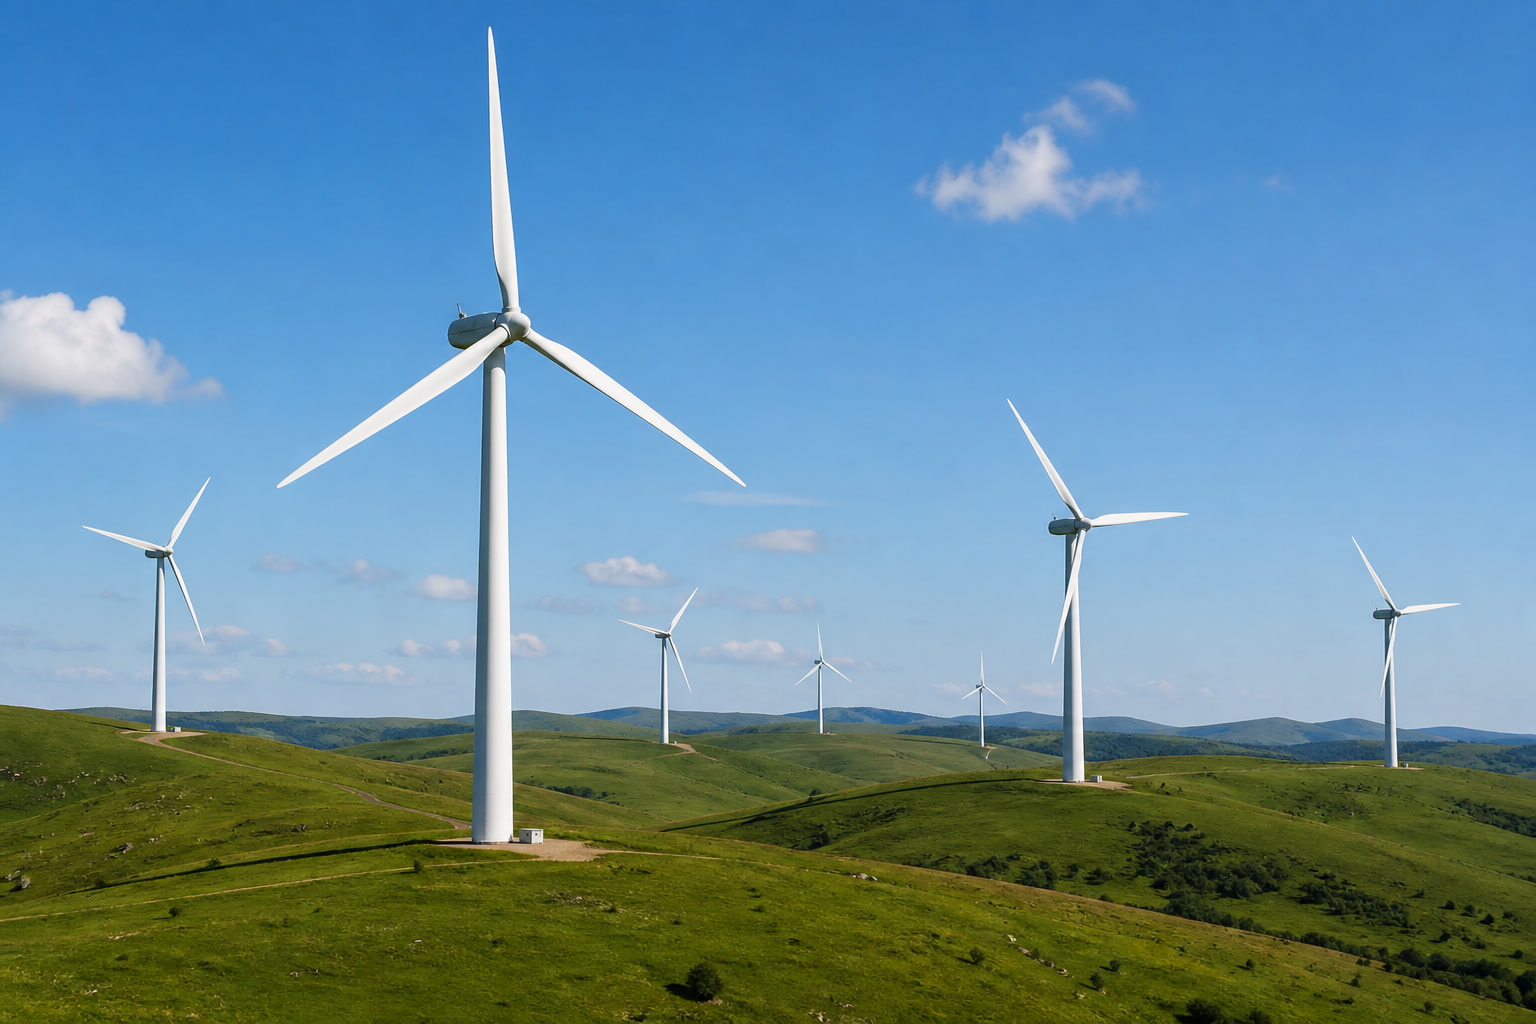
\includegraphics[width=0.58\linewidth]{images/book1/ai/g5-energy-windfarm.jpg}

{\small Uma cadeia de \omterm{def:g5:everyday-energy:energy}{energia} que dá para ver da estrada: o \omterm{def:g2:air-around-us:air}{ar} em movimento gira as pás, e as turbinas mandam \omterm{def:g5:everyday-energy:energy}{energia} elétrica para os fios.}
\end{omfigure}

\section{O Sol na cabeceira da mesa}

\begin{example}[Quase toda cadeia começa no Sol]\label{ex:g5:everyday-energy:sun}
Siga a maioria das cadeias de trás para a frente e você chega ao Sol.
O café da manhã? As plantas o produziram capturando a \omterm{def:g1:light-and-shadows:source}{luz} do Sol; o
seu cereal é sol enlatado. O \omterm{def:g2:air-around-us:wind}{vento}? O Sol aquece as terras de forma
desigual, e o \omterm{def:g2:air-around-us:air}{ar} mexido vira \omterm{def:g2:air-around-us:wind}{vento} --- então até os veleiros
funcionam com \omterm{def:g1:light-and-shadows:source}{luz} do Sol. A lenha? \omterm{def:g1:light-and-shadows:source}{Luz} do Sol guardada pelas árvores.
A água lá em cima da barragem? O Sol a levantou: ele evaporou o mar,
e o vapor virou chuva nas montanhas. Os painéis solares apenas pulam
os intermediários.
\end{example}

\begin{omfigure}
\begin{tikzpicture}[scale=0.85]
  \fill[omThm] (0.9,3.2) circle (0.45);
  \foreach \a in {0,30,...,330} {
    \draw[omThm] (0.9,3.2) ++(\a:0.62) -- ++(\a:0.26);
  }
  \node[below, font=\small] at (0.9,2.5) {o Sol};
  \node[draw, thick, omMeth, font=\small] (p) at (4.3,3.2) {plantas};
  \node[draw, thick, omDef, font=\small] (f) at (7.2,3.2) {alimento};
  \node[draw, thick, omMeth, font=\small] (m) at (9.9,3.2) {músculos};
  \node[draw, thick, omMeth, font=\small] (w) at (4.3,1.4)
    {ar aquecido e mexido};
  \node[draw, thick, omDef, font=\small] (v) at (8.3,1.4)
    {vento e velas};
  \draw[-Stealth, very thick] (1.6,3.2) -- (p);
  \draw[-Stealth, very thick] (p) -- (f);
  \draw[-Stealth, very thick] (f) -- (m);
  \draw[-Stealth, very thick] (1.35,2.75) -- (w);
  \draw[-Stealth, very thick] (w) -- (v);
\end{tikzpicture}

{\small Duas cadeias seguidas até a origem: o café da manhã e o \omterm{def:g2:air-around-us:wind}{vento}
começam os dois no Sol.}
\end{omfigure}

\begin{remark}[Uma palavra que vamos afiar]\label{rem:g5:everyday-energy:promise}
Por enquanto, a \omterm{def:g5:everyday-energy:energy}{energia} é uma história bem contada: reservas, formas,
cadeias. Será que ela pode ser \emph{medida}, como o comprimento em
\omterm{def:g2:measuring-length:units}{metros} e a \omterm{def:g3:measuring-mass:mass}{massa} em \omterm{def:g3:measuring-mass:units}{gramas}? Pode --- a \omterm{def:g5:everyday-energy:energy}{energia} tem uma \omterm{def:g2:measuring-length:measure}{unidade}
própria e uma contabilidade exata, e as duas chegam mais adiante
neste livro, depois que você conhecer direito a velocidade e a \omterm{def:g2:pushes-and-pulls:force}{força}.
As cadeias que você segue neste ano são o mapa; os números virão
morar nele.
\end{remark}

\section{Exercícios}

\begin{exercise}[$\star$]\label{exo:g5:everyday-energy:1}
O que é \omterm{def:g5:everyday-energy:energy}{energia}, nas palavras deste capítulo? Diga quatro coisas que
não podem acontecer sem ela.
\end{exercise}

\begin{exercise}[$\star$]\label{exo:g5:everyday-energy:2}
Ache a reserva: um ratinho de corda correndo; \ um ciclista; \ uma
fogueira; \ um veleiro; \ uma lanterna.
\end{exercise}

\begin{exercise}[$\star$]\label{exo:g5:everyday-energy:3}
Diga cinco formas de \omterm{def:g5:everyday-energy:energy}{energia}, com um exemplo de cada uma tirado do
seu próprio dia.
\end{exercise}

\begin{exercise}[$\star$]\label{exo:g5:everyday-energy:4}
Siga a cadeia de \omterm{def:g5:everyday-energy:energy}{energia} de uma torradeira, como no
\cref{met:g5:everyday-energy:read}: reserva, conversor, formas que
saem.
\end{exercise}

\begin{exercise}[$\star$]\label{exo:g5:everyday-energy:5}
Siga a cadeia do lago de uma barragem até a sua luminária de leitura
hoje à noite.
\end{exercise}

\begin{exercise}[$\star$]\label{exo:g5:everyday-energy:6}
Um celular ``morre''. O que na verdade acabou? Para onde foi essa
\omterm{def:g5:everyday-energy:energy}{energia}, segundo a proposição da cadeia?
\end{exercise}

\begin{exercise}[$\star$]\label{exo:g5:everyday-energy:7}
Por que um notebook esquenta por baixo enquanto você o usa? Qual elo
da cadeia está se mostrando?
\end{exercise}

\begin{exercise}[$\star$]\label{exo:g5:everyday-energy:8}
Mostre que um veleiro funciona com \omterm{def:g1:light-and-shadows:source}{luz} do Sol, seguindo a cadeia dele
de trás para a frente, passo a passo.
\end{exercise}

\begin{exercise}[$\star\star$]\label{exo:g5:everyday-energy:9}
Um inventor anuncia uma luminária que ``não precisa de \omterm{def:g3:first-electric-circuit:battery}{pilha}, nem de
tomada, nem de combustível --- ela simplesmente brilha para
sempre''. Qual lição da \cref{rem:g5:everyday-energy:nofree} o
anúncio desafia? Qual pergunta você deve fazer primeiro ao inventor?
\end{exercise}

\begin{exercise}[$\star\star$]\label{exo:g5:everyday-energy:10}
Uma bola de borracha solta da altura do ombro quica cada vez mais
baixo e por fim fica parada. ``A \omterm{def:g5:everyday-energy:energy}{energia} dela foi destruída'', diz
Leo. Use a \cref{prop:g5:everyday-energy:chain} para defender um
final melhor para a história --- em que forma final a \omterm{def:g5:everyday-energy:energy}{energia} dos
quiques escorregou?
\end{exercise}

\begin{exercise}[$\star\star$]\label{exo:g5:everyday-energy:11}
Algumas casas aquecem água em painéis pretos no telhado; algumas
cozinham com \omterm{def:g1:light-and-shadows:source}{luz} do Sol e espelhos curvos; as células solares
produzem eletricidade a partir da \omterm{def:g1:light-and-shadows:source}{luz} do dia. Explique a frase ``os
painéis solares apenas pulam os intermediários'', do
\cref{ex:g5:everyday-energy:sun}: quais intermediários ficam entre o
Sol e o calor de uma fogueira de lenha?
\end{exercise}
